\subsection{Rotation and Angular Momentum}
From up until this point, we've been dealing in translational motion, where objects move physically from place to place. We're going to reformulate what we've done so far for bodies that only rotate in place, and build up to another conservation law - conservation of angular momentum, the rotational analog to linear momentum. 
\subsubsection{Rotational Kinematics}
When we talk about rotation, we already have the tools to generate kinematic equations for rotation. Instead of position, we have the angle $\theta$ that a body has turned with respect to an axis (which is a unitless scalar quantity). The angular velocity $\omega$ is the time-derivative of the angle $\theta$, similar to the velocity we already know, and angular acceleration $\alpha$ for the time-derivative of the angular velocity, similar to our regular acceleration. Using the same derivations as before for our constant-acceleration kinematic equations, we attain the following: 
\[
	\omega^2 - \omega_0^2 = 2\alpha\Delta\theta
\]
\[
	\theta(t) = \theta_0 + \omega_0 t + \frac{1}{2} \alpha t^2 
\]
One subtlety to note: In three dimensions, which we will soon be using on a regular basis for rotation, angular velocity and acceleration are both vectors that point perpendicular to the velocity and position vectors. Their direction is more specifically specified using the right-hand-rule: that is, as you curl your hand in the direction of the rotation, the thumb should point in the direction of the angular velocity. In fact, we can use the vector cross product to define these vector quantities: 
\[
	\vec v = \vec \omega \times \vec r
\]
\[
	\vec a = \vec \omega \times \vec v + \vec \alpha \times \vec r
\]
These should look somewhat like the formulas we saw for circular motion. The formula for velocity is about the same, just a bit more general if the velocity and position are not perfectly perpendicular to each other. The same is true for the acceleration, where we have that the first term is the centripetal acceleration while the second term is the tangential acceleration. Get comfortable using your right hand. You will see cross products often going forward. 
\subsubsection{Moment of Inertia and Torque}
After considering a rotational analogue for kinematics, we now turn to find a rotational way of describing dynamical systems. To do this, we use the concept of torque on a point particle with respect to a point: 
\[
	\vec \tau = \vec r \times \vec F
\]
where $\vec \tau$ represents the torque on the particle with respect to some point, $\vec r$ the position vector from this arbitrary point to the position of the point particle, and $\vec F$ the net force on that particle. Note that we can use Newton's Second Law, $\vec F = m\vec a$, to substitute in for the force. We can resolve the acceleration into tangential and centripetal components, so we have: 
\begin{align*}
	\vec \tau &= \vec r \times (m \vec a) \\
	&= m \vec r \times (\vec a_c + \vec a_t) \\
	&= m (\vec r \times \vec a_c + \vec r \times \vec a_t) 
\end{align*}
However, since the centripetal acceleration and position vector point in the same direction, their cross product is $0$. For the tangential acceleration, we have $\vec a_t = \vec \alpha \times \vec r$. We can then write the torque as:
\[
	\vec \tau = m \vec r \times \vec alpha \times \vec r
\] 
We can use an expansion of the vector triple product, where $\vec A \times \vec B \times \vec C = \vec B(\vec A \cdot \vec C) - \vec C(\vec A \cdot \vec B)$. Then, we have:
\[
	\vec \tau = m(\vec \alpha (\vec r \cdot \vec r) - \vec r(\vec \alpha \cdot \vec r))
\] 
Noting $\vec \alpha \cdot \vec r = 0$ as $\vec \alpha$ is perpendicular to the plane of rotation, we have:
\[
	\vec \tau = mr^2 \vec \alpha
\]
where $r$ is the distance away from the reference point. For an entire body, we can add up all of these individual torques, noting that the angular acceleration for a rigid body is the same throughout:
\[
	\sum \vec \tau = \sum_i m_i r_i^2 \vec \alpha = I \vec \alpha
\]
This is Newton's Second Law for Rotation. This sum that appears on the right-hand side is called the moment of inertia, denoted $I$, and is taken with respect to an axis of rotation. (For sufficiently symmetric systems, even though we're taking the torque with respect to a point, it can be shown that taking the torque with respect to the entire axis of rotation is equivalent. We'll discuss this when looking at angular momentum.) \\
For discrete systems of point particles, the sum 
\[
	I = \sum_i m_i r_i^2
\]	
for a rigid body is enough to calculate the moment of inertia. However, for large rigid bodies we have to integrate, similar as we did for the center of mass:
\[
	I = \int r^2 \, dm
\]
where $r$ refers to the distance each infinitesimally small part $dm$ is from the reference point. \\
As an example, we'll do a uniform spherical shell with radius $R$ and mass $M$. The surface density $\sigma$ will then just be the mass per unit area, so $\sigma = \frac{M}{4\pi R^2}$. For this 3-D object, let the $y$-axis (directly upward) be the axis of rotation that we're calculating the moment of inertia about. This is a pretty tricky example, which can be done by splitting this shell into rings perpendicular to the axis of rotation. Let $\theta$ be the angle between the positive $y$-axis and the line joining the edge of the ring to the center. This angle ranges from $0$ to $\pi$. \\
\begin{center}
	\begin{asy}
		import solids;
        import three;
        size(7cm);
        real theta = 40;
        currentprojection=orthographic(0.7, -4, 1);
        currentlight=nolight;
        triple center = (0,0,0);
        triple ringctr = (0, 0, Cos(theta));
        real R=1, RS=0.7, inc=100, lat=45, lon=45, tlat=50, tlon=100;
        dot(center);
        real r = 2;
        dot(ringctr);
        revolution Earth=sphere(center, R);  
        triple contact = (Sin(theta), 0, Cos(theta));
        
        draw(surface(Earth), surfacepen=white+opacity(.1), meshpen=0.7*black);
        draw(arc(ringctr, Sin(theta), 90, 180, 90, 0), linewidth(2));
        draw(arc(ringctr, Sin(theta), 90, 0, 90, 180), linewidth(2)+linetype("4 4"));
        draw(center--(Sin(theta), 0, Cos(theta)));
        draw(center--(0,0,R));
        draw(ringctr--contact);
        
        label("$R$", (Sin(theta)/2, 0, Cos(theta)/2), dir(360-theta));
        label("$dM$", contact, dir(40)*1.5);
        label("$\theta$", center, dir(90-(theta/2))*3);
        label("$R \sin\theta$", (Sin(theta)/2, 0, Cos(theta)), dir(90));
	\end{asy}
\end{center}
Now, we need to calculate $dm$ in terms of $\theta$. For any $\theta$, the set of all points on the shell that make an angle of $\theta$ between a radius of that point and the positive $y$-axis is a ring with radius $R\sin \theta$. This ring has "thickness" $R \, d\theta$, which is the length of the arc spanned by a small change $d\theta$ and has a circumference $2 \pi R \sin \theta$. Therefore, the surface area of the ring is $2 \pi R^2 \sin \theta \, d\theta$, and then the mass of the ring is this expression times the surface density, $\sigma$. This gives $dm = 2 \sigma \pi R^2 \sin \theta \, d\theta$. Since the distance from the edge of each ring to the axis is just the radius of each ring, $R \sin \theta$, we can now evaluate the integral:
\begin{align*}
	I &= \int_0^\pi (R \sin \theta)^2 \, dm \\
	&= \int_0^\pi R^2 \sin^2 \theta \cdot 2 \sigma \pi R^2 \sin \theta \, d\theta \\
	&= 2\pi \sigma R^4 \int_0^\pi \sin^3 \theta \, d\theta\\
	&= 2\pi \sigma R^4 \int_{-1}^1 1 - u^2 \, du \\
	&= 2\pi \sigma R^4 \left( u - \frac{1}{3}u^3 \Big|_{-1}^1 \right)	\\
	&= 2 \pi\frac{M}{4\pi R^2}  R^4 \frac{4}{3} = \frac{2}{3}MR^2
\end{align*}
This is a pretty hard example - the trigonometric integral is dealt with by using $\sin^2 \theta = 1 - \cos^2 \theta$ and then substituting $u = \cos \theta$. Also, the setup of $dm$ is hard - one has to realize the "thickness" of the ring not only exists, but also is along the surface of the sphere rather than straight up and down. Calculations don't really get much harder than this, and all the required moments of inertia to know can be derived using a one-dimensional integral. (The most common ones are included as an appendix.)\\
One final thing about moments of inertia: for most cases, such as the sphere we just derived, the axis of rotation will pass through the center of mass, making the derivation for the moment of inertia fairly straightforward. However, there are cases where we will need the axis of rotation to not pass through the center of mass, but through some parallel axis. We can use the aptly-named Parallel Axis Theorem to help with this, which states:
\[
	I_{cm} + Mh^2 = I
\]
where $I$ is the moment of inertia about an axis through some point, $h$ the distance between that point and the center of mass, $M$ the total mass, and $I_{cm}$ the moment of inertia about an axis through the center of mass. The proof of this can be done using calculus, but we will prove it later using energy. 
\subsubsection{Angular Momentum}
Angular momentum is the rotational analog of momentum, defined as follows for a point particle and denoted with the vector $\vec L$:
\[
	\vec L = \vec r \times \vec P
\]
where $\vec r$ is the position of the point particle with respect to some arbitrary point. 
We can take a time derivative of this expression to attain a familiar-looking expression:
\[
	\dv{\vec L}{t} = \dv{}{t}(\vec r \times \vec P) = \dv{\vec r}{t} \times \vec P + \vec r \times \dv{\vec P}{t} = \vec v \times m\vec v + \vec r \times \vec F = \vec r \times \vec F = \vec \tau
\]
The angular momentum of a particle with respect to a point, then, follows all the same rules that linear momentum follows with forces. First, we can now imagine torques as the flow of angular momentum being delivered to and from objects. The angular impulse delivered to a system, then, can be shown to be the change in angular momentum - this is the angular version of the impulse-momentum theorem: 
\[
	\Delta \vec L = \int_{t_1}^{t_2} \vec \tau \, dt
\]
Also, for a system of particles, the time derivative of the total angular momentum of a system of particles with respect to a point is the net external torque on the system:
\[
	\vec \tau_{net} = \dv{\vec L_{sys}}{t}
\]
This can be shown using the same techniques as before with careful consideration of internal and external torques. When no external torques are acting on the system, we know that $\vec L$ is a constant, which gives us the principle of conservation of angular momentum, similar to that for linear momentum: 
\begin{mdframed}[frametitle=Conservation of Angular Momentum]
For a system with no external torques, angular momentum is conserved - the total amount of angular momentum in the system remains constant and is not changed by the internal motion/dynamics of the system.
\end{mdframed}
We'd now like to be able to relate angular momentum to the motion of the center of mass. For a rigid body, the total angular momentum of that object with respect to some arbitrary point is the sum of the angular momenta for each particle within:
\[
	\vec L^{tot} = \sum_i \vec L_i = \sum_i \vec r_i \times \vec P_i = \sum_i \vec r_i \times m_i \vec v_i
\]
where the $\vec r_i$ are the positions of each particle with respect to this arbitrary point, the $\vec v_i$ each particle's velocity, and $m_i$ the mass. \\
Let's force the center of mass into the expression by expressing each position and velocity vector of each particle as the sum of the position/velocity of the center of mass and its position/velocity relative to the center of mass (henceforth referred to as $\vec r_i^*$ and $\vec v_i^*$). Let's plug it all in and distribute the terms:
\begin{align*}
	\vec L^{tot} &= \sum_i (\vec r_{cm} + \vec r_i^*) \times m_i(\vec v_{cm} + \vec v_i^*) \\
	&= \sum_i \vec r_{cm} \times m_i \vec v_{cm} + \sum_i \vec r_{cm} \times m_i \vec v_i^* + \sum_i \vec r_i^* \times m_i \vec v_{cm} + \sum_i \vec r_i^* \times m_i \vec v_i^* 
\end{align*}
These sums all look pretty bad. Let's just take them one at a time. \\
For the first sum, we notice that we can more or less factor out the cross product, and be left with: 
\[
	\sum_i \vec r_{cm} \times m_i \vec v_{cm} = \vec r_{cm} \times \vec v_{cm} \left(\sum_i m_i \right) = \vec r_{cm} \times M\vec v_{cm} = \vec r_{cm} \times \vec P^{tot}
\]
where the total mass of the object is $M$. \\
The second and third sums I claim to be $\vec 0$. This is very tricky to see, but we'll look at the second sum first. First, we can use the fact that the cross product distributes over addition to rearrange the sum, and then we can examine what's left more closely:
\[
	\sum_i \vec r_{cm} \times m_i \vec v_i^*  = \vec r_{cm} \times \sum_i  m_i \vec v_i^*
\]
Where have we seen something similar to this sum before? This looks like the expression for the velocity of the center of mass of an object with respect to some reference point, up to a factor of $M$. However, our reference point IS the center of mass, so this clearly then comes out to be the zero vector. Therefore, 
\[
	\vec r_{cm} \times \sum_i  m_i \vec v_i^* = \vec r_{cm} \times M\vec 0 = \vec 0
\]
Similarly, the sum that appears after rearranging the third sum is the position of the center of mass with respect to the center of mass, which also is the zero vector:
\[
	\sum_i \vec r_i^* \times m_i \vec v_{cm} = \sum_i m_i \vec r_i^* \times \vec v_{cm} = M\vec 0 \times \vec v_{cm} = \vec 0 
\]
The last part is the trickiest part to evaluate. For this, we use the fact that $\vec v_i^* = \vec \omega \times \vec r_i^*$ and $\vec \omega$ is both constant for each particle in the rigid body and perpendicular to the plane that the particle rotates in, as the body rotates about its center of mass: 
\[
	\sum_i \vec r_i^* \times m_i \vec v_i^* = \sum_i m_i (\vec r_i^* \times \vec \omega \times \vec r_i^*) = \sum_i m_i \left[ \vec \omega \left(r_i^*\right)^2 - \vec r_i^*(\vec r_i^* \cdot \vec \omega) \right]  = \sum_i m_i \left(r_i^*\right)^2 \vec \omega
\]
That sum has an expression for the moment of inertia of the rigid body, with respect to its center of mass in it! This now is cleanly written as:
\[
	\sum_i \vec r_i^* \times m_i \vec v_i^* = I_{cm}\vec \omega
\]
So, altogether: 
\[
	\vec L^{tot} = \vec r_{cm} \times \vec P^{tot} + I_{cm} \vec \omega = \vec L^{orb} + \vec L^{spin} 
\]
The first term with the cross product is called the orbital angular momentum (considering how much the object is revolving about the reference point), and the second term is the spin angular momentum (considering how much the object is spinning about its center of mass). Usually, we will pick the reference point so that one of these two terms is zero, more likely than not making the orbital angular momentum zero. For the most part:
\[
	\vec L^{tot} = I_{cm} \vec \omega 
\]
One subtlety is that we normally don't consider angular momentum about a point, but rather an axis of rotation - what we mean by this is that the angular momentum is the same for any point on the axis. This is only true for objects with cylindrical or spherical symmetry, which is sufficient for what we are using it for, but not in the general case. 
\subsubsection{Statics and Rolling Without Slipping}
Armed with the knowledge of rotation, we can look at dynamical systems that are not only moving in space but also rotating. One of the easiest cases is that for systems that are completely at rest, or in a state of static equilibrium. This means that there is no net force on the system, and no net torque. To approach these problems, we will draw extended free-body diagrams, which not only list all of the forces but also show where they act in relation to each other in order to help compute torques. Even though we've seen some statics problems before when discussing forces, be careful to also account for all torques due to gravity (acting at the center of mass) and the torques from contact forces.\\
As an example, consider a long, thin beam of mass $M$ and length $L$, fixed to a vertical wall at a pivot point and at an angle of $\theta$ below the horizontal. An ideal string tied at the end of the beam holds it up, and this string is fixed vertically upwards to the ceiling. We want to find the tension in the string. \\
\begin{center}
	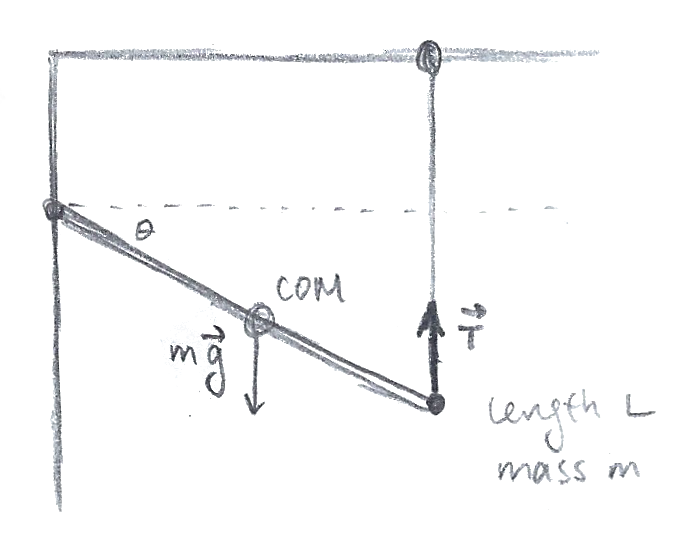
\includegraphics[width=0.4\textwidth]{images/mechintro/statics.png}\\
\end{center}
At first, it seems tempting to just apply Newton's Second Law for all the contact forces and gravity, but quickly it becomes clear that we don't really know how the force from the pivot point really works, and we're missing this information to solve the problem. It's actually much easier to consider the sum of the torques about the pivot point. Since the center of mass of the beam is at the halfway point, the torque due to gravity has magnitude $\tau_g = \frac{L}{2}Mg\cos \theta$. (Make sure you understand why it's cosine and not sine - it's because of the angle between the vectors.) The forces all lie in the same plane, so all the torques run in and out of the page. If we consider up to be the $+y$-direction, right to be the $+x$-direction, and out of the page to be the $+z$-direction (since $\hat x \times \hat y = \hat z$), we have: 
\[
	\sum \tau_z = -\frac{MgL\cos \theta}{2} + \tau_{string} = 0
\]
Therefore, we have that the torque from the string (in the $z$-direction is $\tau_{string} = \frac{MgL\cos \theta}{2}$, since no net torque acts on the system. Noting that $\tau_{string} = TL\cos \theta$, where $T$ is the tension, from this, we can see that the tension $T = \frac{Mg}{2}$. \\
Frequently, aside from using kinematics to look at the system, sometimes we are given that some object or another is rolling without slipping. This means that the following two are true, for a circular object of radius $R$: 
\[
	v_{cm} = \omega R \quad a_{cm} = \alpha R
\]
\begin{center}
	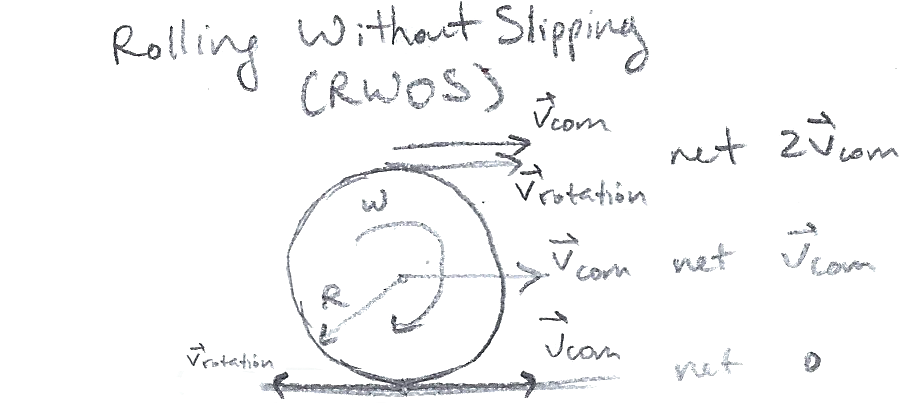
\includegraphics[width=0.4\textwidth]{images/mechintro/rwos.png}\\
\end{center}
When this is true, the frictional force that the object encounters with the ground is actually static and does not change the acceleration of the object. If the object's velocity/angular velocity, etc. do not satisfy these relations, the force of friction will either speed up or slow down the object in order for these two to match so the object starts to roll without slipping. You can see this the next time you go bowling - when you release the ball, the ball slides with constant velocity, but friction begins to turn the ball and it begins to spin faster, and eventually roll normally as the ball travels down the alley. \\
A consequence of the above relations is that relative to the ground, the point in contact with the ground has zero velocity relative to the ground, and the top of the object has speed $2v_{cm}$ relative to the ground. This is very useful to know sometimes - and it can be shown using the principles of relative motion that we discussed in kinematics. \\
Let's revisit Atwood's machine to see how rolling without slipping affects the situation. Consider two masses of $m_1$ and $m_2$ both attached to a taut string ($m_2 > m_1$), wrapped around a solid cylindrical pulley of mass $m_p$ and radius $R$ that is free to spin about its axis. The string does not slip on the pulley, and is still effectively massless. \\
\begin{center}
	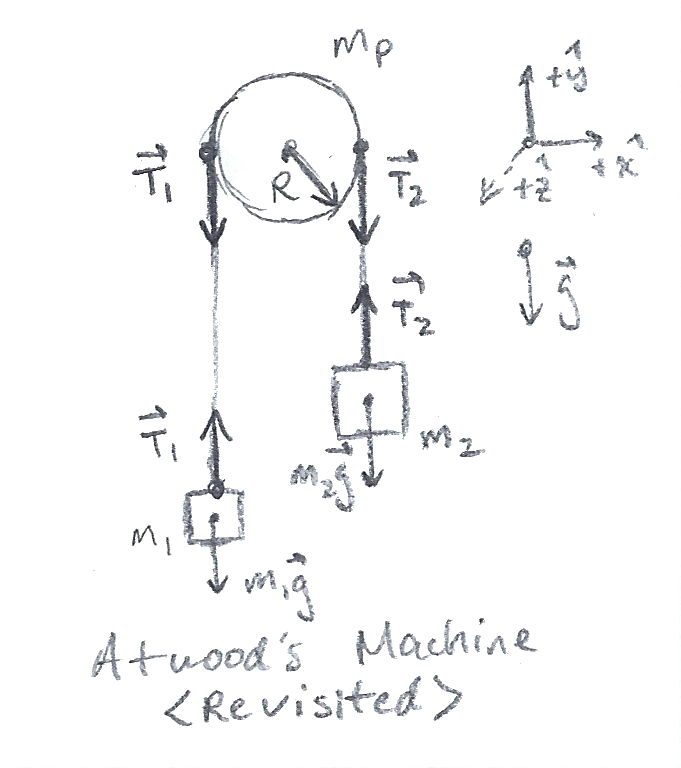
\includegraphics[width=0.4\textwidth]{images/mechintro/atwood-revisited.png}\\
\end{center}
We've drawn an extended free-body diagram to show where each force acts in relation to the objects in the diagram. Notice that the tensions in the strings connecting $m_1$ and $m_2$ to the pulley are not the same, because they're connected to a rotating body now. To distinguish them, let's label the tension on $m_1$ as $T_1$ and the tension on $m_2$ as $T_2$. Let's set up Newton's Second Law, taking into account the force on each of the blocks as well as the torque on the pulley:
\[
	\sum_1 \vec F_i = m_1 \vec g + \vec T_1 = m_1 \vec a
\]
\[
	\sum_2 \vec F_i = m_2 \vec g + \vec T_2 = -m_2 \vec a
\]
\[
	\sum_p \vec \tau_i = \vec R \times \vec T_1 + \vec R \times \vec T_2 = I \vec \alpha
\]
We can project the components of the force in the $+y$-direction (up and down the page), and project the components of the torque along the $+z$-direction (in and out of the page), to get:
\[
	\sum_1 F_y = -m_1g + T_1 = m_1a 
\]
\[
	\sum_2 F_y = -m_2g + T_2 = -m_2a
\]
\[
	\sum_p \tau_z = RT_1 - RT_2 = -I\alpha = -\frac{1}{2}m_pR^2 \alpha
\]
Notice how the sign of the acceleration is reversed for the second block, since we know it's going downwards. Similarly, we've placed a negative sign in front of the angular acceleration since the pulley is rotating clockwise. However, we only have three equations, but we now have four unknowns - the two tensions, the angular acceleration of the pulley, and the acceleration of the blocks. The final thing we need to invoke is the no-slipping condition, which implies the following relation between the angular acceleration of the pulley and the blocks:
\[
	a = R \alpha
\]
We now have all the information we need to solve for the acceleration of the blocks, and the two tensions. Omitting the messy algebra, we have:
\[
	a = \frac{m_2-m_1}{m_1+m_2+\frac{1}{2}m_p}g \quad T_1 = m_1g\frac{4m_2+m_p}{2m_1+2m_2+m_p} \quad T_2 = m_2g\frac{4m_1+m_p}{2m_1+2m_2+m_p} 
\]
Clearly, these expressions are very different than the ones we saw earlier for Atwood's machine, since they now all involve the mass of the pulley from the pulley's moment of inertia.\\
Rolling without slipping problems are a bit more complex, and usually, some information might seem to be missing from the problem in order to solve them. After all, you need to have the same number of variables as equations in order to solve them. If you seem to be missing an equation, it's not a bad idea to impose the rolling without slipping condition on the situation to see if the situation is solvable then. \\
\subsubsection{Summary and Problems}
We now have the tools to look at dynamical systems from a rotational perspective as well as from a translational one. In the following problems, be sure to account for both of these and be able to relate the two different systems of dynamics to each other, with an emphasis on torques, moments of inertia, and angular momentum. \\

\noindent \textbf{Problems}\\
1. (1 $\bigstar$) A uniform cylinder of mass $M$ and radius $R$ has a string wrapped around it. The string is held fixed, and the cylinder falls vertically. a) Show the acceleration of the cylinder is downward with magnitude $a = \frac{2g}{3}$. b) Show the tension in the string $T = \frac{Mg}{3}$. \\
2. (2 $\bigstar$) A uniform solid cylinder of mass $M$ and radius $R$ is at rest on a slab of mass $m$, which in turn rests on a horizontal, frictionless table. If a horizontal force is applied to the slab, it accelerates and the cylinder rolls without slipping. Show the acceleration of the slab is $a = \frac{3F}{3m+M}$.\\
3. (3 $\bigstar$, $\spadesuit$) A uniform horizontal disk of mass $M$ and radius $R$ is spinning about the vertical axis through its center with an angular speed $\omega$. When the spinning disk is dropped onto a horizontal tabletop, kinetic-frictional forces on the disk oppose its spinning motion. Let $\mu_k$ be the coefficient of kinetic friction between the disk and the tabletop. Show that the time required for the disk to stop rotating is $\Delta t = \frac{3R\omega}{4\mu_kg}$. Hint: First, compute the total torque on the disk (from where?) by dividing the disk into thin rings and computing the torque on each ring. \\
4. (2 $\bigstar$) A particle that has a mass $m$ is traveling with a constant velocity along a straight line that is a distance $b$ from the origin $O$. Let $dA$ be the area swept out by the position vector from $O$ to the particle during a time interval $dt$. Show that $\dv{A}{t}$ is constant and is equal to $\frac{L}{2m}$, where $L$ is the magnitude of the angular momentum of the particle about the origin. \\
5. (3 $\bigstar$) A uniform solid sphere with mass $M$ and radius $R$ is set rotating about a horizontal axis at an angular speed $\omega_0$ and then is placed on the floor with its center of mass at rest. If the coefficient of kinetic friction between the sphere and the floor is $\mu_k$ show the speed of the center of mass of the sphere $v = \frac{2R\omega_0}{7}$ when the sphere begins to roll without slipping. \\
6. (4 $\bigstar$) A uniform ladder of length $L$ and mass $m$ leans against a frictionless vertical wall, making an angle of $\theta$ with the horizontal. The coefficient of static friction between the ladder and the ground is $\mu_s$. If your mass is $k$ times that of the ladder, show that the maximum displacement you can move along the ladder $r$ is given by $r = \mu_s L\tan\theta\left(1 + \frac{1}{k}\right) - \frac{L}{2k}$. \\
7. (4 $\bigstar$) A block of mass $M$ rests on a table, connected by a string to a cylindrical (NOT FIXED) pulley of mass $M$ and radius $R$. The string wraps around the pulley and is tied to a block of mass $M$ dangling over the edge of the table. The coefficient of static and kinetic friction between the block on the table and the table is $\frac{1}{2}$. When the system begins moving, the string moves on the cylinder without slipping. Show that the acceleration of each of the blocks is $a = g/5$, and the tensions in the strings are $\frac{4}{5}Mg$ in the string holding the hanging block, and $\frac{7}{10}Mg$ in the string pulling the block along. 
\pagebreak